In this section we report the experimental evaluation of OISVMs
on the place recognition scenario, where the aim is to update
the model to handle variations in an indoor environment due to
human activities over long time spans.

\begin{figure*}[t]
\centering \footnotesize
\begin{tabular}{@{}c@{\hspace{0.002\linewidth}}c@{\hspace{0.002\linewidth}}
c@{\hspace{0.002\linewidth}}c@{\hspace{0.002\linewidth}}
c@{\hspace{0.002\linewidth}}c@{\hspace{0.002\linewidth}}
c@{\hspace{0.002\linewidth}}c@{}}
% -------------------------------------------------------------------
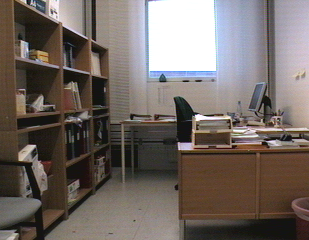
\includegraphics[width=0.123\linewidth]{figs/idol/bo_cloudy.png} &
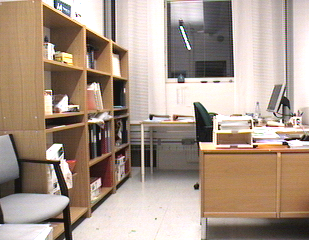
\includegraphics[width=0.123\linewidth]{figs/idol/bo_night.png}  &
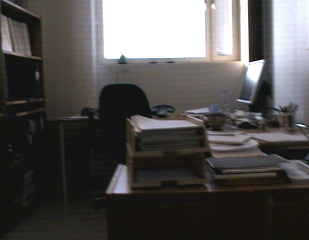
\includegraphics[width=0.123\linewidth]{figs/idol/bo_sunny.png}  &
\includegraphics[width=0.123\linewidth]{figs/idol/cr_cloudy.png} &
\includegraphics[width=0.123\linewidth]{figs/idol/cr_night.png}  &
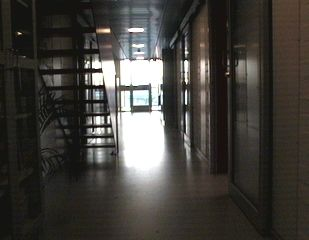
\includegraphics[width=0.123\linewidth]{figs/idol/cr_sunny.png} &
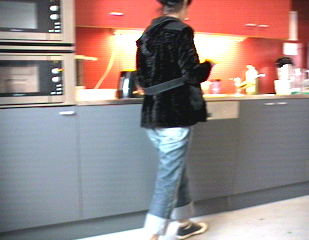
\includegraphics[width=0.123\linewidth]{figs/idol/people1.png}  &
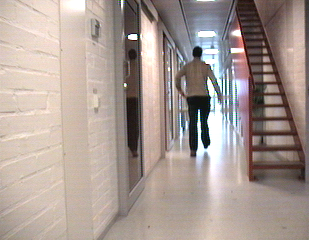
\includegraphics[width=0.123\linewidth]{figs/idol/people2.png}  \\
% -------------------------------------------------------------------
\includegraphics[width=0.123\linewidth]{figs/idol/cup1.png}   &
\includegraphics[width=0.123\linewidth]{figs/idol/cup3.png}   &
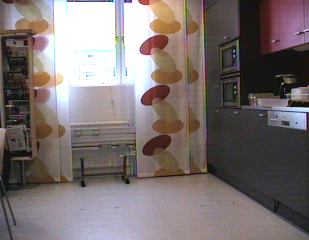
\includegraphics[width=0.123\linewidth]{figs/idol/chair1.png}   &
\includegraphics[width=0.123\linewidth]{figs/idol/chair3.png} &
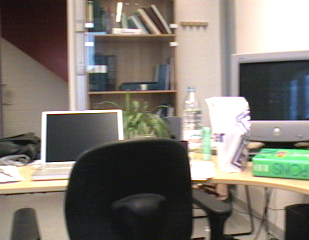
\includegraphics[width=0.123\linewidth]{figs/idol/time1.png} &
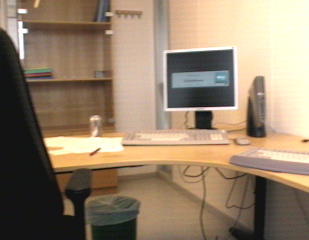
\includegraphics[width=0.123\linewidth]{figs/idol/time2.png} &
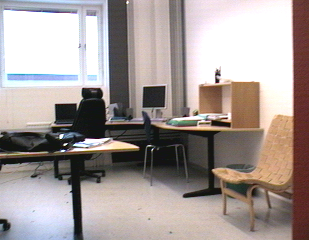
\includegraphics[width=0.123\linewidth]{figs/idol/time3.png}  &
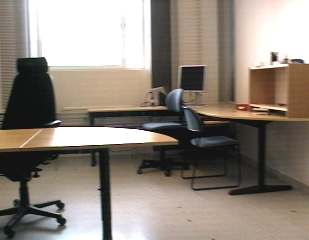
\includegraphics[width=0.123\linewidth]{figs/idol/time4.png}  \\
% -------------------------------------------------------------------
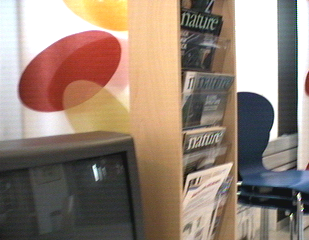
\includegraphics[width=0.123\linewidth]{figs/idol/drive1.png}   &
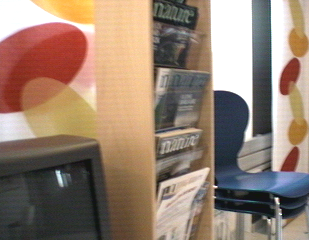
\includegraphics[width=0.123\linewidth]{figs/idol/drive2.png}   &
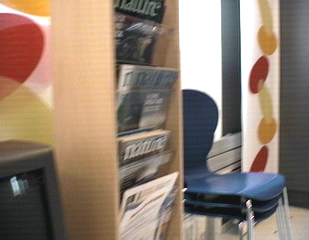
\includegraphics[width=0.123\linewidth]{figs/idol/drive3.png}   &
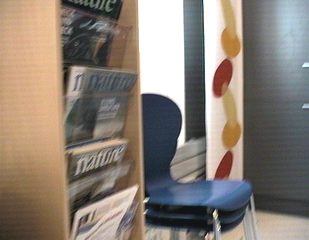
\includegraphics[width=0.123\linewidth]{figs/idol/drive4.png} &
\includegraphics[width=0.123\linewidth]{figs/idol/drive5.png} &
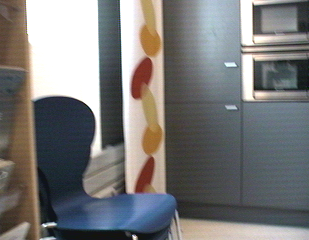
\includegraphics[width=0.123\linewidth]{figs/idol/drive6.png} &
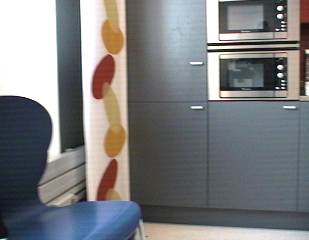
\includegraphics[width=0.123\linewidth]{figs/idol/drive7.png}  &
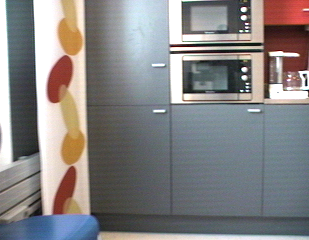
\includegraphics[width=0.123\linewidth]{figs/idol/drive8.png}   \\
% -------------------------------------------------------------------
\end{tabular}
\caption{Sample images illustrating the variations in the IDOL2 database.
Images in the top row show the variability introduced by changes in
illumination as well as people appearing in the environment.
The middle row shows the influence of
people's everyday activity (first four images) as well as larger
variations which happened over a time span of $6$ months. Finally, the
bottom row illustrates the changes in viewpoint observed for a series
of images acquired one after another in $1.6$ seconds.}
\label{fig:idol}
\end{figure*}

Experiments were conducted on the IDOL2 database
(Image Database for rObot Localization 2, \cite{luo:idol2}), which
contains $24$ image sequences acquired using a perspective camera
mounted on two mobile robot platforms, while moving in an indoor
laboratory environment consisting of five different rooms.
The sequences were acquired under various
weather and illumination conditions (sunny, cloudy, and night) and
across a time span of six months. Thus, this data capture natural
variability that occurs in real-world environments because of both
natural changes in the illumination and human activities.
Fig. \ref{fig:idol} shows some sample images from the database,
illustrating the difficulty of the task.  The image sequences in the
database are divided as follows: for each robot platform and for each
type of illumination conditions, there were four sequences
recorded. Of these four sequences, the first two were acquired six
months before the last two. This means that, for each robot and for
every illumination condition, there are always two sequences acquired
under similar conditions, and two sequences acquired under very
different conditions. This makes the database suitable for different
kinds of evaluation on the adaptability of an incremental
algorithm. For further details about the database see \cite{luo:idol2}.

The evaluation was performed using Composed Receptive Field Histograms
(CRFH) \cite{linde:icpr04} as global image features and SIFT descriptors
\cite{lowe99object} of local features computed using a
Harris-Laplace detector \cite{HarrisS88}. In the experiments,
we consider both exponential $\chi^2$ kernel for SVM (when use CRFH),
and local kernels \cite{wallraven:iccv03} (SIFT). Note the kernel in
\cite{wallraven:iccv03} is not always positive semidefinite
\cite{fleuret:bmvc04}, so this is also a test on non-Mercer
kernels that have proved useful for visual recognition.
The kernels used are infinite-dimensional, so for both
kernels we run the OISVM using different values of $\eta$.

OISVMs have been implemented in Matlab and tested against LIBSVM v2.82
\cite{ChangL01}. The software library has been extended to various
families of kernels, and to the fixed-partition incremental SVM \cite{syed99incremental},
an approximate incremental extension of SVM.
In this way we can do a straightforward comparison
between exact and approximate methods
on this task.
Notice that for the standard SVM the training is not online.

The algorithm was trained incrementally on three sequences from IDOL2,
acquired under similar illumination conditions with the same robot
platform; the fourth sequence was used for testing. In order to test
the various properties of interest of the incremental algorithms, we
need a reasonable number of incremental steps.  Thus, every sequence
was split into $5$ subsequences, so that each subset contained one
of the five images acquired by the robot every second (image sequences
were acquired at a rate of 5fps). Since during acquisition the
camera's viewpoint continuously changes \cite{luo:idol2}, the
subsequences could be considered as recorded separately in a static
environment but for varying pose.  This setup allows us to examine how
the algorithms perform on data with less variations. In order to get a
feeling of the variations of the frame images in a sequence, bottom
row of Fig. \ref{fig:idol} shows some sample images acquired within a
time span of 1.6 sec. As a result, training
on each sequence was performed in 5 steps, using one subsequence at a
time, resulting in 15 steps in total. Overall, we considered 36
different permutations of training and test sequences for the
exponential $\chi^2$ kernel and 36 permutations for the matching
kernel; here we report average results with standard
deviation. Fig. \ref{fig:exp:idol}, left, shows the recognition rates
of the exponential $\chi^2$ kernel (top) and matching kernel (bottom)
experiments obtained at each step using OISVM, the fixed-partition
algorithm and the standard SVM. Fig. \ref{fig:exp:idol}, right,
reports the number of support vectors stored in the model at each step
of the incremental procedure, for both kernel types.

We see that, performance-wise, all methods achieves statistically
comparable results; this is true for both kernel types. As far the
machine size is concerned, the OISVM algorithm shows a considerable
advantage with respect to the fixed-partition method. In the case of the exponential
$\chi^{2}$ kernel this advantage is truly impressive (Fig
\ref{fig:exp:idol}, top right): for $\eta=0.017$ and $0.025$ the
size at the final incremental step is $34\%/22\%$ of that of the
fixed-partition method and $28\%/18\%$ of that of the
standard batch method. Even more important, OISVM, for these two
values of $\eta$, has found a plateau in memory, while for other
methods the trend seems to be of a growth proportional to the
number of training data. Note
that the choice of the parameter $\eta$ is crucial for achieving an
optimal trade-off between compactness of the solution and optimal
performance.

It is very interesting to note that, in the case of the matching
kernel, the memory reduction for OISVM is less pronounced, and there
is not a clear plateau in memory growth by any of the algorithms.
This behavior might be due to several factors: to begin with, the
matching kernel is not a Mercer kernel \cite{fleuret:bmvc04}, which
might affect the algorithm. Also, the algorithm does not reach a
plateau in the SVs growth because, in the induced space of the
matching kernel, there seems to be a high probability that pair of
training points are orthogonal, or almost orthogonal, to each other
(notice that, as the kernel is not a Mercer one, the geometric
interpretation might not be valid). Anyway, given enough training
points, the machine will always reach a maximum size and will stop
growing \cite{engel2004}.Other tests on a set of standard databases commonly used in the
machine learning community, as well as more details about OISVM can be
found in \cite{Orabona07}.

It is worth noting that, even if the solution is kept small and the
number of support vectors will be finite in any case, the algorithm
must store all the training samples that it receives. This can be a
problem in an online setting, but it could be solved using, for
example, some kind of forgetting strategy. Another strategy can be the
use out-of-core storage of the data (i.e., storage on the hard disk)
in order to be able to deal with big training sets.

\begin{figure*}[t]
  \centering \footnotesize
  \begin{tabular}{c@{\hspace{0.5cm}}c}
  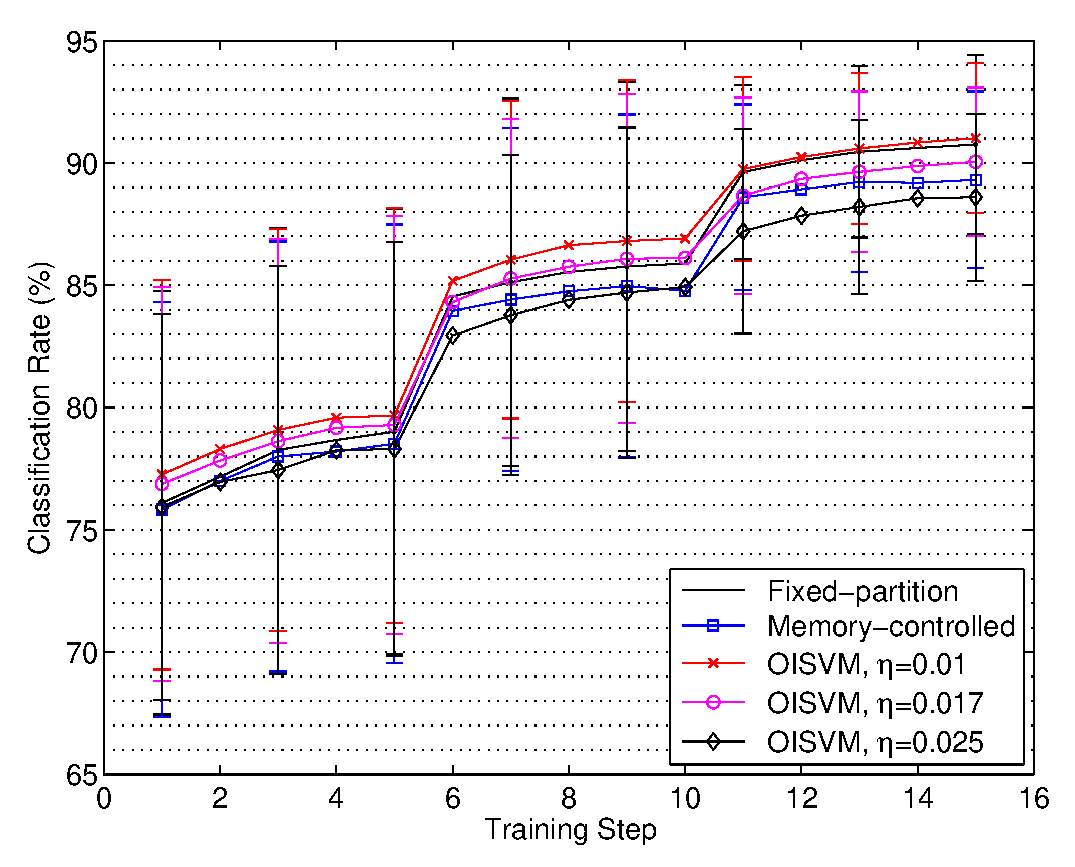
\includegraphics[width=0.47\linewidth]{figs/results/chi_cr} &
  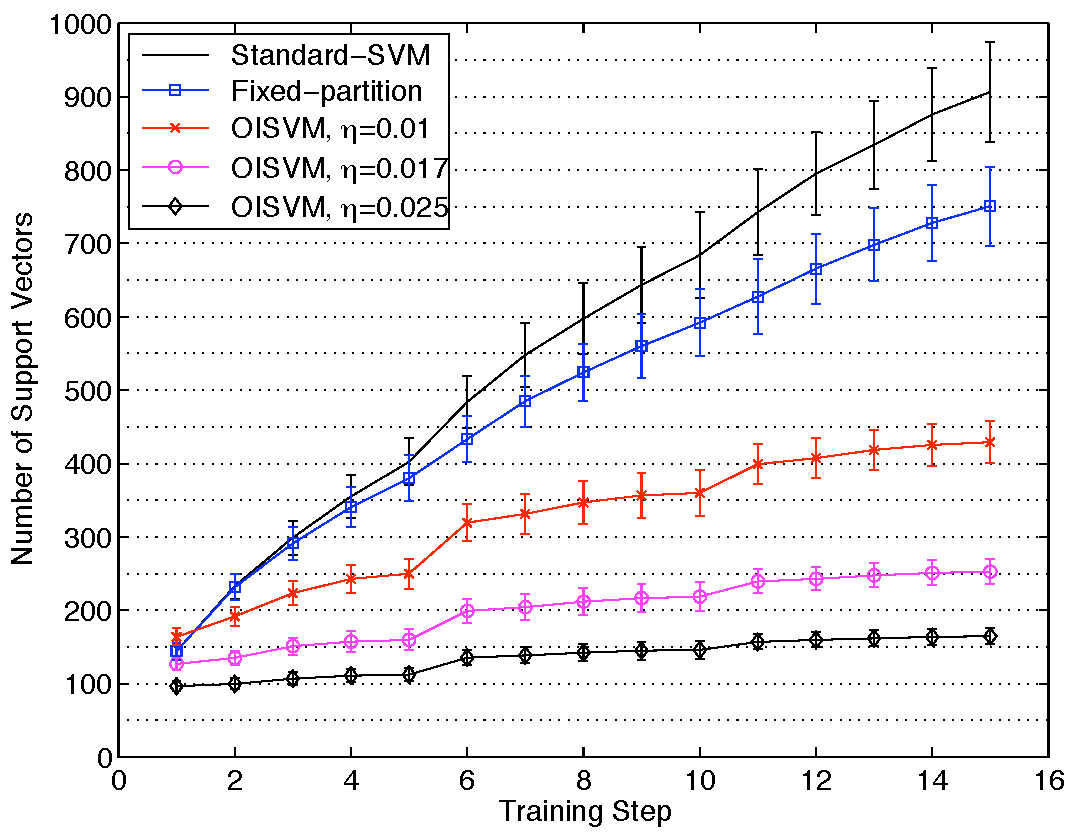
\includegraphics[width=0.47\linewidth]{figs/results/chi_sv} \vspace{0.1cm}\\
  \multicolumn{2}{c}{(a)~Number of support vectors and classification rate obtained at each incremental step using $\chi^2$ kernel.}  \\
  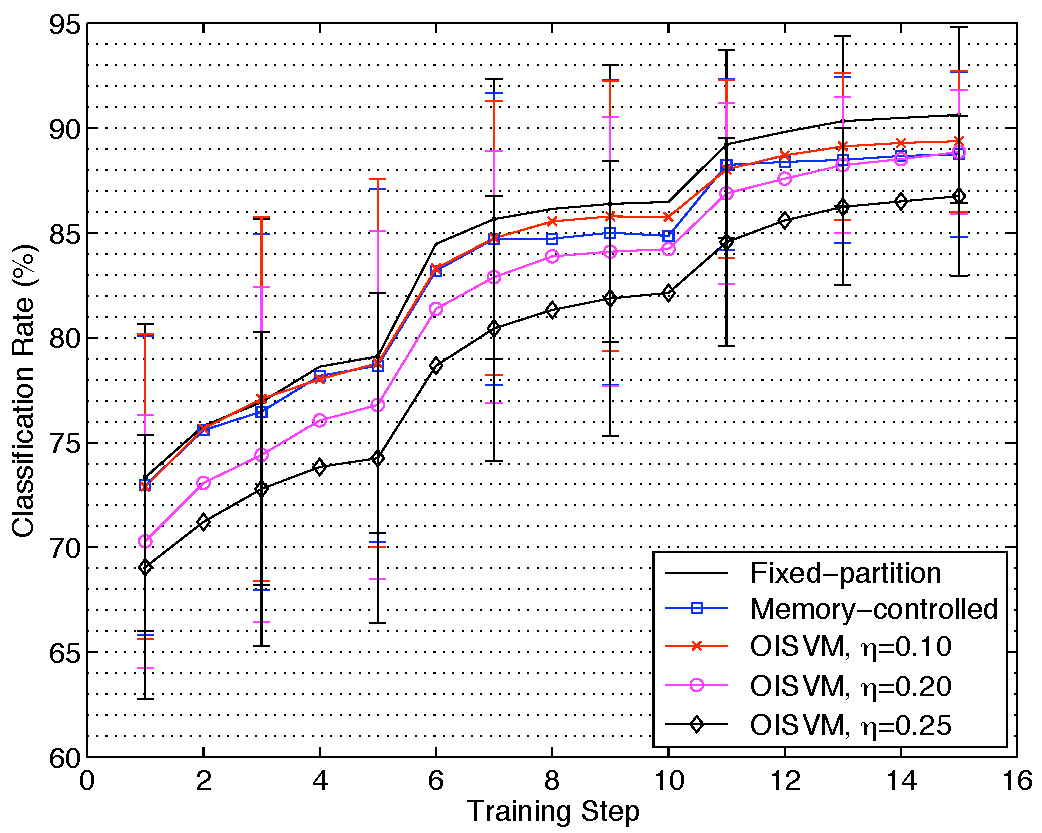
\includegraphics[width=0.47\linewidth]{figs/results/local_cr} &
  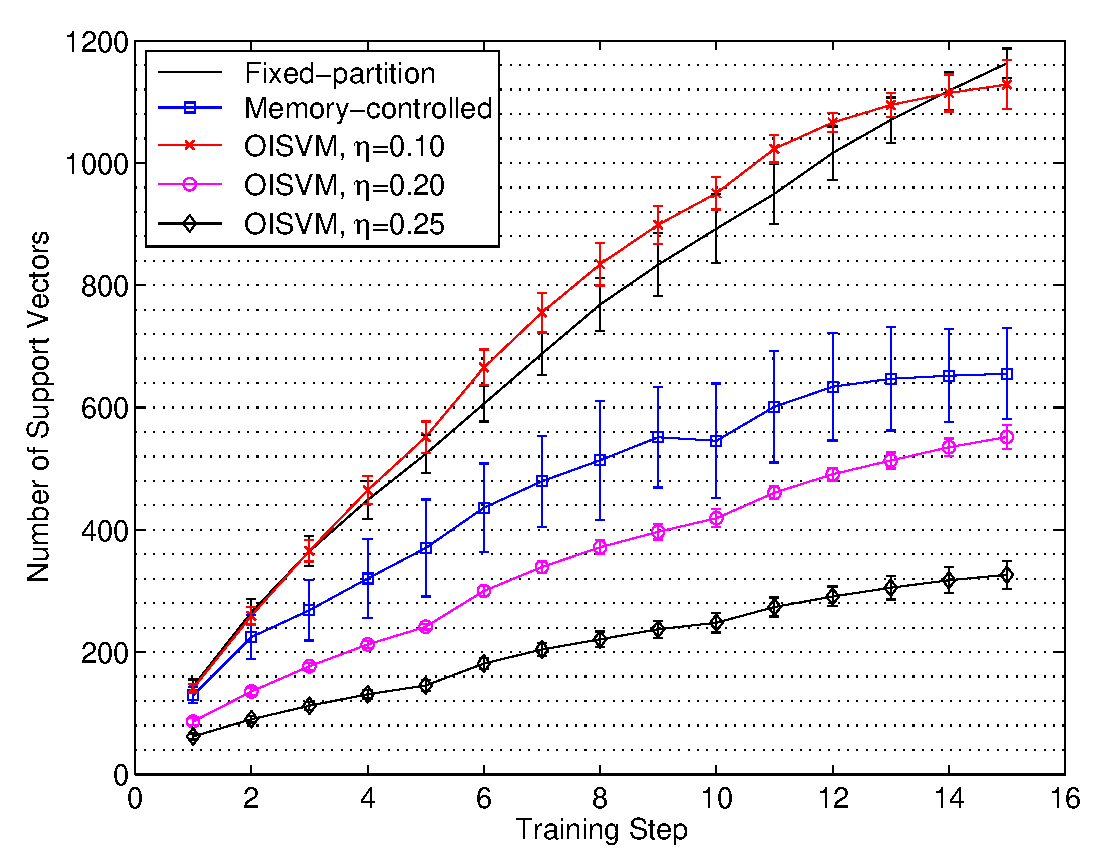
\includegraphics[width=0.47\linewidth]{figs/results/local_sv} \vspace{0.1cm}\\
  \multicolumn{2}{c}{(b)~Number of support vectors and classification rate obtained at each incremental step using local kernel.} \\
  \end{tabular}
\caption{Average results obtained for experiment performed on the IDOL2 database, using
         OISVM with three different values of $\eta$, the fixed-partition and the standard SVM.
         These figures are best viewed in color.}
\label{fig:exp:idol}
\end{figure*}
